\capitulo{5}{Aspectos relevantes del desarrollo del proyecto}

En este capítulo se explicarán las partes más importantes del desarrollo del proyecto.

\section{Desarrollo de la aplicación web}

Para realizar la primera fase del desarrollo, la recogida de los datos, se ha desarrollado una aplicación web que permitiese grabar a los pacientes durante la realización de los ejercicios de rehabilitación mientras son dirigidos por el personal especializado.

Esta aplicación se ha compuesto de dos partes. Una ha consistido en el diseño y consecuente implementación de una interfaz hombre-máquina fácil de usar y accesible mediante un mando sencillo\footnote{Concretamente un mando de la consola SNES adaptado para ser usado mediante USB}. Esta se compone de una serie de botones de colores, directamente relacionados con los del mando~(figuras~\ref{fig:help} y \ref{fig:menu_paciente}), que permiten iniciar una comunicación mediante videoconferencia con el personal terapéutico como finalizar la reunión. Durante el proceso de la llamada el vídeo del paciente es capturado y enviado al servidor para su procesado posterior.

\begin{figure}
	\centering
	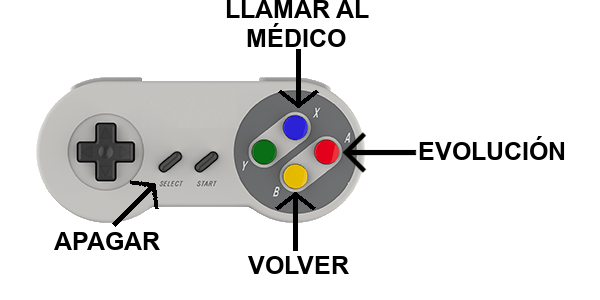
\includegraphics[width=\textwidth]{img/ayuda.png}
	\caption{Funcionamiento del mando de SNES para el control de la aplicación web por parte del paciente.}
	\label{fig:help}
\end{figure}

\begin{figure}
	\centering
	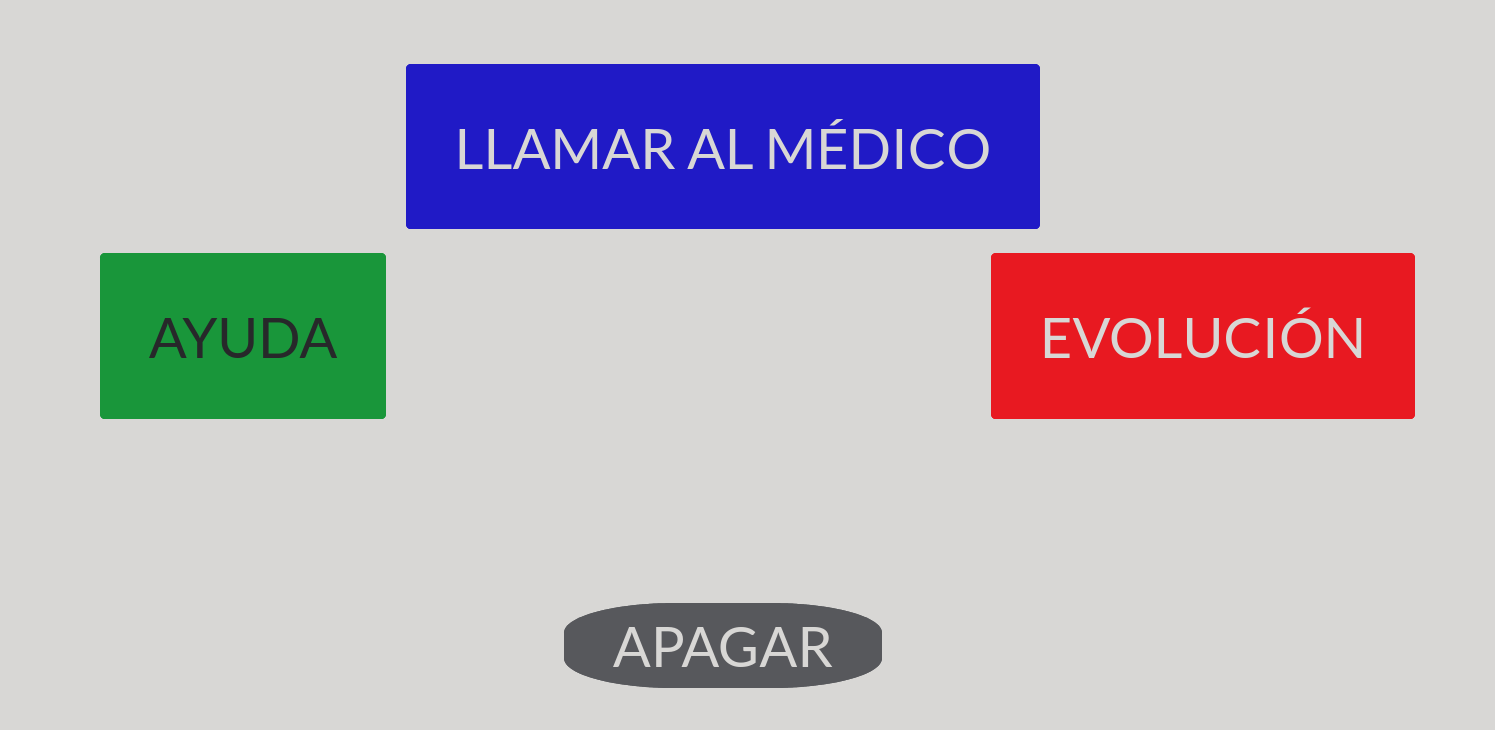
\includegraphics[width=\textwidth]{img/menu_paciente.png}
	\caption{Menú del paciente}
	\label{fig:menu_paciente}
\end{figure}

La segunda parte consiste en la interfaz del terapeuta encargado de dirigir las sesiones de rehabilitación del paciente ofreciendo una interfaz sencilla que permite conectarse a las videoconferencias de los diferentes pacientes y dirigir las sesiones de terapia además de gestionar la evolución del paciente~(figura~\ref{fig:menu_respon}).

\begin{figure}
	\centering
	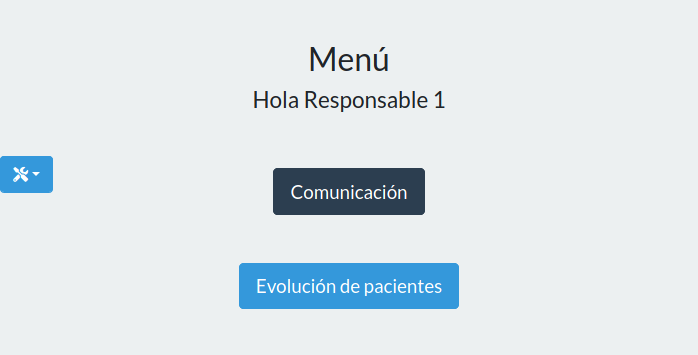
\includegraphics[width=\textwidth]{img/menu_responsable.png}
	\caption{Menú del terapeuta}
	\label{fig:menu_respon}
\end{figure}


TODO: Quizás sería interesante explicar las valoraciones otorgadas de la aplicación si se tienen antes de la entrega del trabajo. 

TODO: Comentar las características de hardware de los dispositivos de despliegue